\section{Rayonnement dipolaire électrique}

Le rayonnement électromagnétique est un phénomène fondamental. Toute charge en mouvement accéléré rayonne un champ [$\vec{E},\vec{B}$] et donc de l'énergie électromagnétique.

\subsection{Le modèle du dipôle électrique oscillant}

On a une distribution neutre, et on fait l'hypothèse que les charges mobiles sont en mouvement sinusoïdal. Par exemple, un atome possède une charge $q>0$ fixe (le noyau) et une charge $-q<0$ mobile (électrons). On peut donc le modéliser avec un dipôle comme à la Figure~\ref{fig:modelisation_atome_dipole_oscillant}. Dans ce cas, le mouvement est~$z(t)=z_{0}\cos(\omega t)$ où $z_{0}$ est la distance typique entre le noyau et l'électron, et le moment dipolaire est donc
\begin{equation*}
    \boxed{
        \vec{p}(t)=q\vec{G^{-}O}(t)=-qz_{0}\cos(\omega t)\vec{u_{z}}.
    }
\end{equation*}

\begin{figure}
    \centering
    \tikzsetnextfilename{modelisation_atome_dipole_oscillant}
    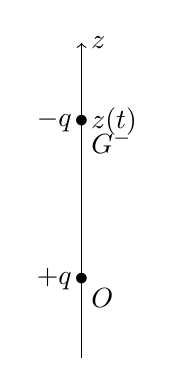
\begin{tikzpicture}[scale=1]  
        % \helpgrid{3}{3}
        \draw[->] (0,0)--++(0,4) node [right] {$z$};
        \node at (0,3) {$\bullet$};
        \node at (0,3) [left] {$-q$};
        \node at (0,3) [right] {$z(t)$};
        \node at (0,3) [below right] {$G^{-}$};
        \node at (0,1) {$\bullet$};
        \node at (0,1) [left] {$+q$};
        \node at (0,1) [below right] {$O$};
    \end{tikzpicture}
    \caption{Modélisation d'un atome par un dipôle électrique oscillant.}    
    \label{fig:modelisation_atome_dipole_oscillant}
\end{figure}

En ordre de grandeur, on a $p_{0}\sim 10^{-29}\si{\coulomb\metre}$ (environ 1 Debye), et $\omega\sim 10^{15}\si{\radian\per\second}$. Pour une antenne, on a $f\sim 100\si{\mega\hertz}$ d'où $\lambda\sim 3\si{\metre}$. Ainsi, la longueur d'une antenne est typiquement de l'ordre de la longueur d'onde.

\subsection{Les trois échelles de longueur}

On a accès à trois longueurs : $z_{0}$ qui est la longueur typique entre la charge positive et la charge négative, $\lambda=c/f$ qui est la longueur d'onde de l'onde sinusoïdale, et $r$ qui est la distance de l'observateur au dipôle.

Plusieurs hypothèses permettent de distinguer ces trois longueurs:
\begin{itemize}
    \item \textbf{Approximation dipolaire} : $z_{0}\ll r$;
    \item \textbf{Mouvement des charges non relativiste} : la vitesse maximale entre les deux charges doit être bien plus petite que la vitesse de la lumière, d'où $\omega z_{0}\ll c$, ce qui revient, comme $c/\omega = \lambda/(2\pi)$, à $z_{0}\ll\lambda$.
    \item \textbf{Champ lointain ou zone de rayonnement} : on suppose le phénomène de propagation prépondérant, et donc le temps de propagation est très grand devant la période du dipôle, d'où $r/c\gg T$ (c'est l'inverse de l'ARQS), d'où $r\gg cT=\lambda$.
\end{itemize}

Ainsi, on a
\begin{equation*}
    \boxed{
        z_{0}\ll \lambda\ll r.
    }
\end{equation*}

\subsection{Champ électromagnétique dans la zone de rayonnement : approche qualitative}